\documentclass[aspectratio=169,12pt]{beamer}
\usepackage[utf8]{inputenc}
\usepackage[T1]{fontenc}
\usepackage{amsmath, amssymb}
\usepackage{booktabs}
\usepackage{colortbl}
\usepackage{hyperref}
\usepackage{makecell}
\usepackage{ragged2e}
\usepackage{bytefield}
\usepackage{tikz}
\usetikzlibrary{arrows.meta, positioning, shapes.geometric, calc, tikzmark, shapes.misc, matrix}
\usepackage{tcolorbox}
\usepackage{pgfplots}
\pgfplotsset{compat=1.17}

\usetheme{Madrid}
\usecolortheme{default}

% Custom colors
\definecolor{mygreen}{RGB}{0,128,0}
\definecolor{myblue}{RGB}{0,0,255}
\definecolor{myred}{RGB}{255,0,0}

\title{Computer Structure}
\subtitle{236267}
\author{Lihu Rappoport}
\date{}

\begin{document}

\frame{\titlepage}

% Table of Contents
\begin{frame}{Outline}
\tableofcontents
\end{frame}

\section{Course Overview}

% Slide 2: General Course Information
\begin{frame}{General Course Information}
\begin{itemize}
    \item \textbf{Grade}
    \begin{itemize}
        \item 20\% : 3 exercises (all mandatory) -- submission in pairs
        \item 80\% final exam
    \end{itemize}
    \item \textbf{Come to the lectures and to the tutorials !}
    \begin{itemize}
        \item The material for the exam includes \underline{all} that is taught during the lectures and the tutorials -- the foils do not contain everything
    \end{itemize}
    \item \textbf{Course web site}
    \begin{itemize}
        \item \url{http://webcourse.cs.technion.ac.il/236267/}
        \item Foils will be on the web several days before each lecture
    \end{itemize}
\end{itemize}
\end{frame}

% Slide 3: Class Focus
\begin{frame}{Class Focus}
\begin{itemize}
    \item \textbf{CPU}
    \begin{itemize}
        \item Introduction: performance, instruction set (RISC vs. CISC)
        \item Pipeline, hazards
        \item Branch prediction
        \item Out-of-order execution
    \end{itemize}
    \item \textbf{Memory Hierarchy}
    \begin{itemize}
        \item Cache and cache coherency
        \item Main memory
        \item Virtual Memory
    \end{itemize}
    \item \textbf{More topics}
    \begin{itemize}
        \item Multi-threading
        \item System
        \item Power considerations
    \end{itemize}
\end{itemize}
\end{frame}

\section{Computer Architecture Basics}

% Slide 4: Personal Computer System
\begin{frame}{Personal Computer System}
\hspace*{0cm}%
\begin{tikzpicture}[
    icon/.style={inner sep=0pt},
    lbl/.style={font=\scriptsize\bfseries},
    bus/.style={draw, thick, <->, >=Stealth},
    busname/.style={font=\tiny, fill=white, inner sep=1pt}
]
    % CPU - center top
    \node[icon] (cpu) {\includegraphics[height=1.2cm]{figures/noun-cpu-8157304.png}};
    \node[lbl, above=0.02cm of cpu] {CPU};

    % RAM - left of CPU
    \node[icon, left=2.5cm of cpu] (ram) {\includegraphics[height=1.1cm]{figures/noun-ram-7483151.png}};
    \node[lbl, above=0.02cm of ram] {Memory};

    % NVMe SSD - below left of CPU (fast storage via CPU PCIe)
    \node[icon, below left=1.3cm and 2cm of cpu] (nvme) {\includegraphics[height=0.9cm]{figures/noun-nvme-6849180.png}};
    \node[lbl, below=0.02cm of nvme] {SSD (NVMe)};

    % GPU - right of CPU
    \node[icon, right=2cm of cpu] (gpu) {\includegraphics[height=1cm]{figures/noun-graphics-card-1036913.png}};
    \node[lbl, above=0.02cm of gpu] {Graphics Card};

    % Display - right of GPU
    \node[icon, right=1.5cm of gpu] (display) {\includegraphics[height=1.2cm]{figures/noun-computer-screen-8056981.png}};
    \node[lbl, above=0.02cm of display] {Display};

    % Chipset/PCH - below CPU
    \node[icon, below=1.3cm of cpu] (pch) {\includegraphics[height=1.1cm]{figures/noun-chipset-7648727.png}};
    \node[lbl, left=0.1cm of pch] {Chipset};

    % HDD - below right of chipset (slow storage via SATA)
    \node[icon, below right=0.7cm and 1.5cm of pch] (hdd) {\includegraphics[height=0.85cm]{figures/noun-hard-drive-7483169.png}};
    \node[lbl, below=0.02cm of hdd] {HDD};

    % Network card - right of chipset
    \node[icon, right=1.8cm of pch] (nic) {\includegraphics[height=0.85cm]{figures/noun-network-card-7443121.png}};
    \node[lbl, below=0.02cm of nic] {Network};

    % USB Hub - below chipset
    \node[icon, below=1.2cm of pch] (usb) {\includegraphics[height=0.75cm]{figures/noun-usb-8182582.png}};
    \node[lbl, below=0.02cm of usb] {USB Hub};

    % Keyboard - below left of USB hub
    \node[icon, below left=0.4cm and 0.8cm of usb] (kbd) {\includegraphics[height=0.65cm]{figures/noun-keyboard-8103038.png}};
    \node[lbl, left=0.05cm of kbd] {Keyboard};

    % Mouse - below right of USB hub
    \node[icon, below right=0.4cm and 0.8cm of usb] (mouse) {\includegraphics[height=0.65cm]{figures/noun-mouse-8184967.png}};
    \node[lbl, right=0.05cm of mouse] {Mouse};

    % Connections - CPU direct
    \draw[bus] (cpu) -- node[busname, above] {Memory Bus} (ram);
    \draw[bus] (cpu) -- node[busname, above] {PCIe} (gpu);
    \draw[bus] (cpu) -- node[busname, left, pos=0.4] {PCIe} (nvme);
    \draw[bus] (gpu) -- node[busname, above] {HDMI/DP} (display);

    % CPU to Chipset
    \draw[bus] (cpu) -- node[busname, left] {DMI} (pch);

    % Chipset to peripherals
    \draw[bus] (pch) -- node[busname, right, pos=0.5] {SATA} (hdd);
    \draw[bus] (pch) -- node[busname, above] {PCIe} (nic);
    \draw[bus] (pch) -- node[busname, left] {USB} (usb);

    % USB hub to peripherals
    \draw[bus] (usb) -- node[busname, left, pos=0.5] {} (kbd);
    \draw[bus] (usb) -- node[busname, right, pos=0.5] {} (mouse);

\end{tikzpicture}

\begin{tikzpicture}[remember picture, overlay]
    \node[anchor=south east, text width=6cm, font=\scriptsize, align=left,
          fill=yellow!20, rounded corners=3pt, inner sep=4pt]
        at ([xshift=-0.5cm, yshift=0.3cm]current page.south east) {
        \textit{Modern PCs are complex---and this is before discussing what's \textbf{inside} the CPU: multiple cores, caches, system agent... That will be our focus.}
    };
\end{tikzpicture}
\end{frame}

% Slide 5: Architecture & Microarchitecture
\begin{frame}{Architecture \& Microarchitecture}
\begin{itemize}
    \item \textbf{\textcolor{mygreen}{Architecture}}\\
    The processor features seen by the ``user''
    \begin{itemize}
        \item Instruction set, addressing modes, data width, \ldots
    \end{itemize}
    \vspace{0.3cm}
    \item \textbf{\textcolor{myblue}{Micro-architecture}}\\
    The internal implementation of a processor
    \begin{itemize}
        \item Caches size and structure, number of execution units, \ldots
    \end{itemize}
    \vspace{0.3cm}
    \item Processors with different $\mu$Arch can support the same architecture
    \vspace{0.3cm}
    \item \textbf{Compatibility}
    \begin{itemize}
        \item A new processor can run existing software
        \item The processor $\mu$Arch is new, but it supports the Architecture of past generations, possibly adding to it
    \end{itemize}
\end{itemize}
\end{frame}

\section{Performance Metrics}

% Slide 6: MOSFET Scaling
\begin{frame}{Moore's Law: Transistor Count Doubles Every Two Years}
\centering
\begin{tikzpicture}
    % Background: Transistor count PNG image - sized to fit frame
    \node[anchor=center, inner sep=0] (image) at (0,0) {
        \includegraphics[width=\textwidth,height=0.85\textheight,keepaspectratio]{figures/Transistor-Count-over-time-cropped.png}
    };
    
    % Overlay: MOSFET scaling plot on top of the image - full width
    \begin{scope}
        \begin{semilogyaxis}[
            at={(image.south west)},
            anchor=south west,
            width=0.77\textwidth,
            height=0.85\textheight,
            xmin=1962, xmax=2025,
            ymin=-1000, ymax=10000,
            hide x axis,
            hide y axis,
            legend pos=north east,
            legend style={font=\scriptsize, fill=white, fill opacity=0.8, draw=red!80!black, yshift=1.2cm, xshift=-4.5cm},
            axis background/.style={fill=none}
        ]
        % MOSFET scaling data points with labels
        \addplot[
            red, 
            very thick, 
            mark=*, 
            mark size=2pt, 
            mark options={fill=red},
            nodes near coords,
            point meta=explicit symbolic,
            every node near coord/.append style={
                font=\tiny,
                text=red!80!black,
                anchor=south
            }
        ] coordinates {
            (1971, 10000) [10$\mu$m]
            (1974, 6000) [6$\mu$m]
            (1977, 3000) [3$\mu$m]
            (1981, 1500) [1.5$\mu$m]
            (1984, 1000) [1$\mu$m]
            (1987, 800) [800nm]
            (1990, 600) [600nm]
            (1993, 350) [350nm]
            (1996, 250) [250nm]
            (1999, 180) [180nm]
            (2001, 130) [130nm]
            (2003, 90) [90nm]
            (2005, 65) [65nm]
            (2007, 45) [45nm]
            (2009, 32) [32nm]
            (2012, 22) [22nm]
            (2014, 14) [14nm]
            (2016, 10) [10nm]
            (2018, 7) [7nm]
            (2020, 5) [5nm]
            (2022, 3) [3nm]
            (2025, 2) [2nm]
        };
        \addlegendentry{MOSFET Feature Size}
        \end{semilogyaxis}
    \end{scope}
\end{tikzpicture}
\end{frame}

% Slide 7: CPU Performance
\begin{frame}{CPU Performance}
\begin{itemize}
    \item \textbf{CPUs work according to a clock signal}
    \begin{itemize}
        \item Clock \textcolor{myblue}{\textbf{cycle}} is measured in nsec ($10^{-9}$ of a second)
        \item Clock frequency (= $\frac{1}{\text{clock cycle}}$) measured in GHz ($10^9$ \textcolor{myblue}{\textbf{cyc}}/sec)
    \end{itemize}
    \vspace{0.3cm}
    \item \textbf{CPI -- \textcolor{myblue}{Cycles} Per \textcolor{mygreen}{Instruction}}
    \begin{itemize}
        \item Average \#\textcolor{myblue}{\textbf{cycles}} per \textcolor{mygreen}{\textbf{Instruction}} (in a given program)
        \item IPC (= $\frac{1}{\text{CPI}}$) : \textcolor{mygreen}{\textbf{Instructions}} per \textcolor{myblue}{\textbf{cycles}}
    \end{itemize}
\end{itemize}

\vspace{0.3cm}
\begin{alertblock}{CPI Definition}
\centering
$$\text{CPI} = \frac{\text{Total number of \textcolor{myblue}{\textbf{cycles}} required to execute the program}}{\text{Total number of \textcolor{mygreen}{\textbf{instructions}} executed in the program}}$$
\end{alertblock}
\end{frame}

% Slide 8: Calculating the CPI of a Program
\begin{frame}{Calculating the CPI of a Program}
\begin{itemize}
    \item $IC_i$: \#times instruction of type $i$ is executed in the program
    \item IC: \#instruction executed in the program: $IC = \sum_{i=1}^{n} IC_i$
    \item $F_i$: relative frequency of instruction of type $i$: $F_i = \frac{IC_i}{IC}$
    \item $CPI_i$ -- \#cycles to execute instruction of type $i$
    \begin{itemize}
        \item e.g.: $CPI_{add} = 1$, $CPI_{mul} = 3$
    \end{itemize}
    \item \#cycles required to execute the entire program:
    $$\#cyc = \sum_{i=1}^{n} CPI_i \times IC_i = CPI \times IC$$
    \item CPI:
    $$CPI = \frac{\#cyc}{IC} = \frac{\sum_{i=1}^{n} CPI_i \times IC_i}{IC} = \sum_{i=1}^{n} CPI_i \times \frac{IC_i}{IC} = \sum_{i=1}^{n} CPI_i \times F_i$$
\end{itemize}
\end{frame}

% Slide 9: CPU Time
\begin{frame}{CPU Time}
\begin{itemize}
    \item \textbf{CPU Time} - time required to execute a program
    \begin{center}
    \Large
    \colorbox{yellow!20}{CPU Time = IC $\times$ CPI $\times$ clock cycle}
    \end{center}
    \vspace{0.5cm}
    \item \textbf{Our goal: minimize CPU Time}
    \begin{itemize}
        \item Minimize clock cycle: more GHz (process, circuit, uArch)
        \item Minimize CPI: \hspace{1.5cm} uArch (e.g.: more execution units)
        \item Minimize IC: \hspace{2cm} architecture (e.g.: vector instructions)
    \end{itemize}
\end{itemize}
\end{frame}

% Slide 10: Amdahl's Law
\begin{frame}{Amdahl's Law}
Suppose enhancement E accelerates a fraction F of the task by a factor S, and the remainder of the task is unaffected, then:

\vspace{0.3cm}
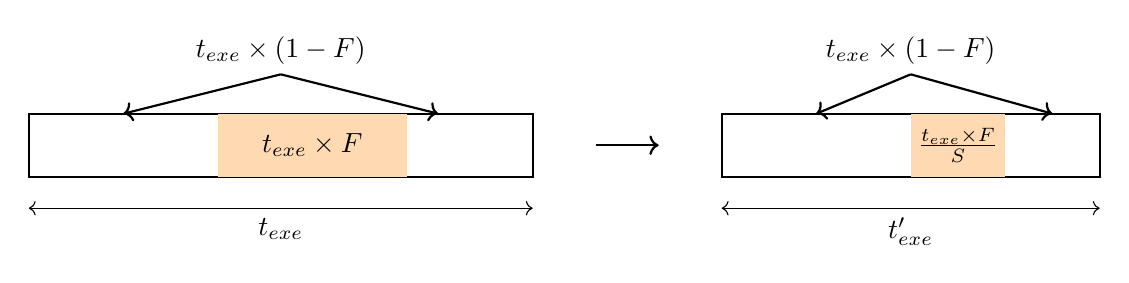
\begin{tikzpicture}[scale=0.8]
    % Original execution
    \draw[thick] (0,1) rectangle (8,2);
    \fill[orange!30] (3,1) rectangle (6,2);
    \node at (4.5,1.5) {$t_{exe} \times F$};
    \draw[<->] (0,0.5) -- (8,0.5) node[midway, below] {$t_{exe}$};
    
    % Label for (1-F) parts with arrows
    \node (label1) at (4,3) {$t_{exe} \times (1-F)$};
    \draw[->, thick] (label1.south) -- (1.5,2);
    \draw[->, thick] (label1.south) -- (6.5,2);
    
    % Arrow
    \draw[->, thick] (9,1.5) -- (10,1.5);
    
    % Enhanced execution
    \draw[thick] (11,1) rectangle (17,2);
    \fill[orange!30] (14,1) rectangle (15.5,2);
    \node at (14.75,1.5) {$\frac{t_{exe} \times F}{S}$};
    \draw[<->] (11,0.5) -- (17,0.5) node[midway, below] {$t'_{exe}$};
    
    % Label for (1-F) parts with arrows
    \node (label2) at (14,3) {$t_{exe} \times (1-F)$};
    \draw[->, thick] (label2.south) -- (12.5,2);
    \draw[->, thick] (label2.south) -- (16.25,2);
\end{tikzpicture}

\vspace{-0.2cm}
$$t'_{exe} = t_{exe} \times \left[(1-F) + \frac{F}{S}\right]$$

$$\text{Speedup}_{overall} = \frac{t_{exe} - t'_{exe}}{t_{exe}} = 1 - \left[(1-F) + \frac{F}{S}\right] = F - \frac{F}{S}$$
\end{frame}

% Slide 11: Amdahl's Law Example
\begin{frame}{Amdahl's Law: Example}
\begin{itemize}
    \item Floating point instructions improved to run 2$\times$ faster
    \item 10\% of the executed instructions are FP instruction
\end{itemize}

\vspace{0.5cm}
$$t'_{exe} = t_{exe} \times \left(0.9 + \frac{0.1}{2}\right) = 0.95 \times t_{exe}$$

$$\text{Speedup}_{overall} = 1 - 0.95 = 0.05 = 5\%$$

\vspace{1cm}
\begin{alertblock}{Corollary}
\centering
\Large Make The Common Case Fast
\end{alertblock}
\end{frame}

\section{Performance Evaluation}

% Slide 12: Evaluating Performance of future CPUs
\begin{frame}{Evaluating Performance of future CPUs}
\begin{itemize}
    \item \textbf{Use a performance simulator to evaluate the performance of a new feature / algorithm}
    \begin{itemize}
        \item Models the uarch to a great detail
        \item Run 100's of representative applications
    \end{itemize}
    \item \textbf{Produce the performance s-curve}
    \begin{itemize}
        \item Sort the applications according to the IPC increase
        \item Baseline (0) is the processor without the new feature
    \end{itemize}
\end{itemize}

\begin{columns}
\column{0.5\textwidth}
\centering
\textbf{S-curve with negative results}\\
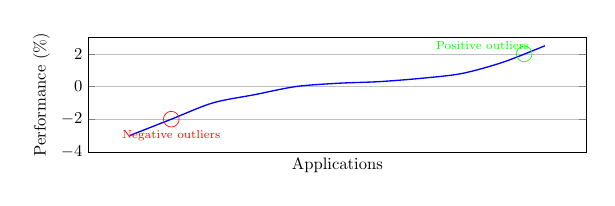
\begin{tikzpicture}[scale=0.6]
    \begin{axis}[
        xlabel={Applications},
        ylabel={Performance (\%)},
        width=\textwidth,
        height=4cm,
        ymin=-4, ymax=3,
        grid=major,
        xtick=\empty
    ]
    \addplot[blue, thick, smooth] coordinates {
        (0,-3) (10,-2) (20,-1) (30,-0.5) (40,0) (50,0.2) 
        (60,0.3) (70,0.5) (80,0.8) (90,1.5) (100,2.5)
    };
    \node[red, circle, draw] at (axis cs:10,-2) {};
    \node[red] at (axis cs:10,-3) {\scriptsize Negative outliers};
    \node[green, circle, draw] at (axis cs:95,2) {};
    \node[green] at (axis cs:85,2.5) {\scriptsize Positive outliers};
    \end{axis}
\end{tikzpicture}

\column{0.5\textwidth}
\centering
\textbf{S-curve of a good feature}\\
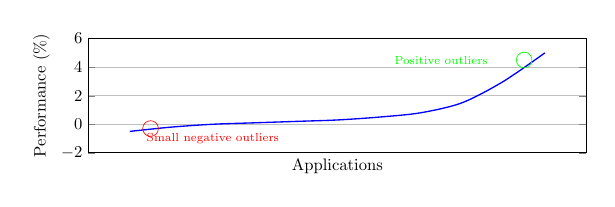
\begin{tikzpicture}[scale=0.6]
    \begin{axis}[
        xlabel={Applications},
        ylabel={Performance (\%)},
        width=\textwidth,
        height=4cm,
        ymin=-2, ymax=6,
        grid=major,
        xtick=\empty
    ]
    \addplot[blue, thick, smooth] coordinates {
        (0,-0.5) (10,-0.2) (20,0) (30,0.1) (40,0.2) (50,0.3) 
        (60,0.5) (70,0.8) (80,1.5) (90,3) (100,5)
    };
    \node[red, circle, draw] at (axis cs:5,-0.3) {};
    \node[red] at (axis cs:20,-1) {\scriptsize Small negative outliers};
    \node[green, circle, draw] at (axis cs:95,4.5) {};
    \node[green] at (axis cs:75,4.5) {\scriptsize Positive outliers};
    \end{axis}
\end{tikzpicture}
\end{columns}
\end{frame}

% Slide 13: Using Benchmarks for Comparing Performance
\begin{frame}{Using Benchmarks for Comparing Performance}
\textbf{Benchmark types:}
\begin{itemize}
    \item Real applications, or representative parts of real apps
    \item Synthetic benchmarks which represent typical workloads
\end{itemize}

\vspace{0.1cm}
\textbf{Benchmarks are targeted at specific system usages:}

\begin{columns}[T]
\column{0.48\textwidth}
\textbf{SPEC INT} -- Integer applications:
\begin{itemize}
    \scriptsize
    \item Data compression
    \item C compiler
    \item Perl interpreter
    \item Database system
    \item Chess-playing
    \item Text-processing
\end{itemize}

\textbf{SYSMark} -- Business usage patterns:
\begin{itemize}
    \scriptsize
    \item Office: Acrobat, Excel, PowerPoint, Word
    \item Media: Photoshop, Premiere, Sketchup
    \item Analysis: Excel, WinZip
\end{itemize}

\column{0.48\textwidth}
\textbf{SPEC FP} -- Floating point applications:
\begin{itemize}
    \scriptsize
    \item Fluid dynamics
    \item Quantum chemistry
    \item Image ray-tracing
    \item Speech recognition
\end{itemize}

\vspace{0.3cm}
\textbf{TPC Benchmarks}
\begin{itemize}
    \scriptsize
    \item Transaction-processing throughput and database performance
\end{itemize}

\end{columns}
\end{frame}

\section{Instruction Set Architecture}

% Slide 14: Instruction Set Design
\begin{frame}{Instruction Set Design}
\begin{columns}[c]
\column{0.48\textwidth}
\centering
\begin{tikzpicture}[
    box/.style={draw, thick, minimum width=4cm, minimum height=0.8cm, font=\small\bfseries, rounded corners=4pt},
    icon/.style={inner sep=0pt},
    lbl/.style={font=\scriptsize}
]
    % Software layer
    \node[box, fill=blue!15] (sw) at (0,0) {Software};

    % ISA layer (the contract) - two lines
    \node[box, fill=yellow!40, minimum height=0.9cm, align=center, below=0.5cm of sw] (isa) {Instruction Set\\Architecture};

    % Hardware layer
    \node[box, fill=green!15, below=0.5cm of isa] (hw) {Hardware};

    % Software side icons - centered on Software box corners
    \node[icon] (progicon) at (sw.north west) {%
        \includegraphics[height=0.85cm]{figures/noun-programmer-8008262.png}};
    \node[icon] (compicon) at (sw.north east) {%
        \includegraphics[height=0.85cm]{figures/noun-compiler-5057301.png}};

    % Labels for software side
    \node[lbl, above=0.02cm of progicon] {Programmer};
    \node[lbl, above=0.02cm of compicon] {Compiler};

    % Hardware side icon - centered on Hardware box corner
    \node[icon] (cpuicon) at (hw.south west) {%
        \includegraphics[height=0.85cm]{figures/noun-cpu-8157304.png}};
    \node[lbl, below=0.02cm of cpuicon] {CPU};

    % Bidirectional arrows between layers (the interface)
    \draw[<->, very thick, red!70!black] (sw.south) -- (isa.north);
    \draw[<->, very thick, red!70!black] (isa.south) -- (hw.north);
\end{tikzpicture}

\column{0.52\textwidth}
\small
\textbf{The ISA is a \textcolor{red}{contract}:}
\vspace{0.15cm}
\begin{itemize}\setlength{\itemsep}{2pt}
    \item \textbf{What software sees:}
    \begin{itemize}\setlength{\itemsep}{0pt}
        \scriptsize
        \item Instructions \& opcodes
        \item Registers
        \item Addressing modes
        \item Data types \& widths
    \end{itemize}
    \item \textbf{What hardware provides:}
    \begin{itemize}\setlength{\itemsep}{0pt}
        \scriptsize
        \item Executes all ISA instructions
        \item Implementation hidden
    \end{itemize}
\end{itemize}

\vspace{0.15cm}
\begin{alertblock}{\small Compatibility}
\scriptsize
Different $\mu$Arch can support the \textbf{same} ISA\\
$\Rightarrow$ old software runs on new CPUs
\end{alertblock}
\end{columns}
\end{frame}

% Slide 15: ISA Considerations
\begin{frame}{ISA Considerations}
\begin{itemize}\setlength{\itemsep}{0.4cm}
    \item \textbf{Reduce IC} $\Rightarrow$ reduce execution time
    \begin{itemize}
        \item Example: a single vector instruction replaces multiple scalar instructions
    \end{itemize}

    \item \textbf{Simple instructions} $\Rightarrow$ simpler HW implementation
    \begin{itemize}
        \item Higher frequency, lower power, lower cost
    \end{itemize}

    \item \textbf{Minimize code size} $\Rightarrow$ faster fetch, smaller memory footprint
    \begin{itemize}
        \item Long instructions increase fetch time and cache pressure
        \item Critical for workloads with large code footprints
    \end{itemize}
\end{itemize}

\vspace{0.4cm}
\begin{alertblock}{Trade-off}
These goals often conflict: reducing IC may require complex instructions, which increase code size and HW complexity
\end{alertblock}
\end{frame}

% Slide 16: Architectural Consideration Example
\begin{frame}{Architectural Consideration Example}
\begin{itemize}
    \item \textbf{Most instructions use short immediate values}
    \item Supporting only the maximum size for all instructions wastes code space
    \item \textbf{Solution:} Variable-length immediates or multiple instruction formats
\end{itemize}

\vspace{0.2cm}
\centering
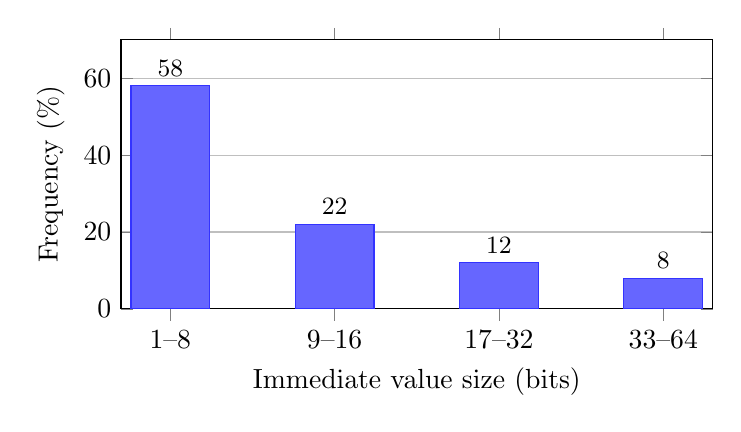
\begin{tikzpicture}
    \begin{axis}[
        ybar,
        xlabel={Immediate value size (bits)},
        ylabel={Frequency (\%)},
        width=0.75\textwidth,
        height=5cm,
        ymin=0, ymax=70,
        symbolic x coords={1--8, 9--16, 17--32, 33--64},
        xtick=data,
        nodes near coords,
        nodes near coords align={vertical},
        every node near coord/.append style={font=\small},
        bar width=1cm,
        grid=major,
        ymajorgrids=true,
        xmajorgrids=false,
        fill=blue!60
    ]
    \addplot[fill=blue!60, draw=blue!80] coordinates {
        (1--8, 58) (9--16, 22) (17--32, 12) (33--64, 8)
    };
    \end{axis}
\end{tikzpicture}

\vspace{0.1cm}
\small 80\% of immediates fit in 16 bits or less
\end{frame}

% Slide 17: ISA Extensions for Reducing IC
\begin{frame}{ISA Extensions for Reducing IC (Instruction Count)}
\textbf{Example:} 128-bit packed (vector) / scalar single precision FP (4$\times$32)

\begin{columns}
\column{0.5\textwidth}
\centering
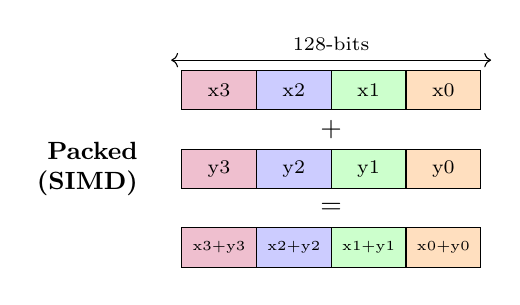
\begin{tikzpicture}[node distance=0.5cm,
    reg/.style={matrix of nodes, ampersand replacement=\&,
        nodes={draw, minimum width=0.95cm, minimum height=0.5cm, font=\scriptsize, anchor=center},
        column sep=-\pgflinewidth,
        column 1/.style={nodes={fill=purple!25}},
        column 2/.style={nodes={fill=blue!20}},
        column 3/.style={nodes={fill=green!20}},
        column 4/.style={nodes={fill=orange!25}}}
]
    \matrix[reg] (X) { x3 \& x2 \& x1 \& x0 \\ };
    \node[below of=X] (plus) {+};
    \matrix[reg, below of=plus] (Y) { y3 \& y2 \& y1 \& y0 \\ };
    \node[below of=Y] (eq) {=};
    \matrix[reg, below of=eq, nodes={font=\tiny}] (R) { x3+y3 \& x2+y2 \& x1+y1 \& x0+y0 \\ };
    \draw[<->] (X.north west) -- (X.north east) node[midway, above] {\scriptsize 128-bits};
    \node[left=0.3cm of Y, anchor=east, align=right, font=\small\bfseries] {Packed\\(SIMD)};
\end{tikzpicture}

\column{0.5\textwidth}
\centering
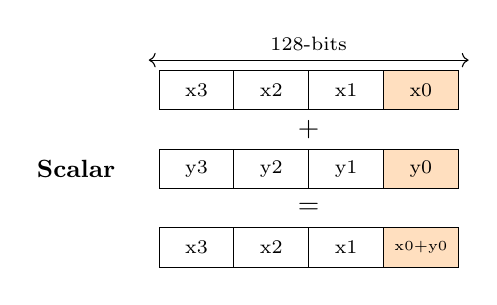
\begin{tikzpicture}[node distance=0.5cm,
    reg/.style={matrix of nodes, ampersand replacement=\&,
        nodes={draw, minimum width=0.95cm, minimum height=0.5cm, font=\scriptsize, anchor=center},
        column sep=-\pgflinewidth},
    colored/.style={column 4/.style={nodes={fill=orange!25}}}
]
    \matrix[reg, colored] (X) { x3 \& x2 \& x1 \& x0 \\ };
    \node[below of=X] (plus) {+};
    \matrix[reg, colored, below of=plus] (Y) { y3 \& y2 \& y1 \& y0 \\ };
    \node[below of=Y] (eq) {=};
    \matrix[reg, colored, below of=eq] (R) { x3 \& x2 \& x1 \& |[font=\tiny]| x0+y0 \\ };
    \draw[<->] (X.north west) -- (X.north east) node[midway, above] {\scriptsize 128-bits};
    \node[left=0.3cm of Y, anchor=east, font=\small\bfseries] {Scalar};
\end{tikzpicture}
\end{columns}

\vspace{0.4cm}
\begin{itemize}
    \item A single ``packed add'' instruction replaces 4 ``add'' instructions
    \item Requires HW support: execution unit that performs ``packed add'' in a single cycle
\end{itemize}
\end{frame}

% Slide 18: CISC Processors
\begin{frame}[fragile]{CISC Processors}
\begin{itemize}
    \item \textbf{CISC -- Complex Instruction Set Computer} -- a high-level machine language
    \begin{itemize}
        \item Example: x86
    \end{itemize}
    \item \textbf{Complex instructions and complex addressing modes}\\
    $\Rightarrow$ complicates the processor and slows down the simple, common instructions\\
    $\Rightarrow$ contradicts \emph{Make The Common Case Fast}
    \item \textbf{Small number of registers} $\Rightarrow$ requires many memory accesses
    \item \textbf{Non-orthogonal registers}: some operations supported only on specific registers\\
    $\Rightarrow$ Not compiler friendly
    \item \textbf{ALU operations directly on memory}
    \begin{verbatim}
    add  eax, 7680[ecx] ;eax ← MEM[7680+ecx]+ eax
    \end{verbatim}
    \item \textbf{Variable length instructions}
    \begin{itemize}
        \item Common instructions get short codes $\Rightarrow$ save code length
        \item Difficult to decode few instructions in parallel: only after an instruction is decoded, its length (and when the next instruction starts) is known
        \item An instruction may cross a cache line or a page
    \end{itemize}
\end{itemize}
\end{frame}

% Slide 19: Top 10 Instructions
\begin{frame}{Top 10 Instructions}
\centering
\begin{table}
\begin{tabular}{clr}
\toprule
\textbf{Rank} & \textbf{instruction} & \textbf{\% of total executed} \\
\midrule
1 & load & 22\% \\
2 & conditional branch & 20\% \\
3 & compare & 16\% \\
4 & store & 12\% \\
5 & add & 8\% \\
6 & and & 6\% \\
7 & sub & 5\% \\
8 & move register-register & 4\% \\
9 & call & 1\% \\
10 & return & 1\% \\
\midrule
& \textbf{Total} & \textbf{96\%} \\
\bottomrule
\end{tabular}
\end{table}

\vspace{0.5cm}
\begin{alertblock}{Key Observation}
\centering
Simple instructions dominate instruction frequency
\end{alertblock}
\end{frame}

% Slide 20: CISC vs RISC - Philosophy
\begin{frame}{CISC vs RISC: Fundamental Philosophy}
\begin{columns}[T]
\column{0.52\textwidth}
\begin{block}{CISC}
\textbf{Complex Instruction Set Computer}
\begin{itemize}
    \item High-level machine language
    \item Single instruction does a lot of work
    \item "Make assembly programming easier"
    \item Example: x86 (Intel, AMD)
\end{itemize}
\end{block}

\column{0.03\textwidth}
% Empty column for spacing

\column{0.40\textwidth}
\begin{block}{RISC}
\textbf{Reduced Instruction Set Computer}
\begin{itemize}
    \item Simple, uniform instructions
    \item Each instruction does one thing
    \item "Make hardware fast and simple"
    \item Example: ARM, RISC-V, MIPS
\end{itemize}
\end{block}
\end{columns}

\vspace{0.5cm}
\begin{alertblock}{The Core Trade-off}
\begin{itemize}
    \item \textbf{CISC Problem:} Complex instructions slow down simple, common operations
    \item \textbf{RISC Solution:} Simple instructions $\Rightarrow$ fast hardware
    \item \textbf{Key Principle:} "\emph{Make The Common Case Fast}" -- simple instructions dominate
\end{itemize}
\end{alertblock}
\end{frame}

% Slide 21: RISC vs CISC Detailed Comparison
\begin{frame}{RISC vs CISC: Detailed Comparison}
\centering
\begin{table}
\resizebox{0.95\textwidth}{!}{%
\begin{tabular}{l|l|l}
\toprule
\textbf{Aspect} & \textbf{CISC} & \textbf{RISC} \\
\midrule
\textbf{Instruction Set} & \textcolor{red}{Large, complex} & \textcolor{mygreen}{Small, simple} \\
\textbf{Instruction Length} & \textcolor{red}{Variable (1-15 bytes in x86)} & Fixed (e.g., 32 bits) \\
\textbf{Addressing Modes} & \textcolor{red}{Many complex modes} & \textcolor{mygreen}{Few simple modes} \\
\midrule
\textbf{Memory Access} & ALU operations on memory & Load/Store architecture only \\
& \texttt{add eax, [mem]} & Separate load, compute, store \\
\midrule
\textbf{Registers} & \textcolor{red}{Few (8-16)}, non-orthogonal & \textcolor{mygreen}{Many (32+)}, \textcolor{mygreen}{orthogonal} \\
& Special purpose registers & \textcolor{mygreen}{General purpose registers} \\
\textbf{Instruction Form} & Two-address: \texttt{add dst, src} & Three-address: \texttt{add dst, src1, src2} \\
\midrule
\textbf{Execution Time} & \textcolor{red}{Variable (1-100+ cycles)} & \textcolor{mygreen}{Uniform (mostly 1 cycle)} \\
\textbf{Code Size} & \textcolor{mygreen}{Smaller (dense encoding)} & \textcolor{red}{Larger (simple encoding)} \\
\textbf{Compiler} & \textcolor{red}{Complex, harder to optimize} & \textcolor{mygreen}{Simple, easier to optimize} \\
\textbf{Hardware Complexity} & \textcolor{red}{Complex control logic} & \textcolor{mygreen}{Simple control logic} \\
\textbf{Design Time} & \textcolor{red}{Longer time-to-market} & \textcolor{mygreen}{Shorter time-to-market} \\
\textbf{Die Space for Cache} & \textcolor{red}{Less room} & \textcolor{mygreen}{More room} \\
\bottomrule
\end{tabular}
}
\end{table}
\vspace{0.2cm}
\footnotesize
\textcolor{mygreen}{Green} = Advantage, \textcolor{red}{Red} = Disadvantage
\end{frame}

% Slide 22: Modern Processor Reality
\begin{frame}{Modern Processor Reality: Convergence}
\begin{itemize}
    \item \textbf{Modern CISC processors use RISC $\mu$-arch ideas}
    \begin{itemize}
        \item Internally translate CISC instructions into RISC-like micro-operations
        \item The inside core looks much like that of a RISC processor
        \item Example: Intel x86 $\rightarrow$ micro-ops (uops)
    \end{itemize}
    \vspace{0.5cm}
    \item \textbf{RISC processors are not "pure" RISC anymore}
    \begin{itemize}
        \item Support division which takes many cycles
        \item Modern ARM has complex SIMD instructions
        \item Some have variable-length instruction modes (ARM Thumb)
    \end{itemize}
    \vspace{0.5cm}
    \item \textbf{Benefits of simple architecture remain}
    \begin{itemize}
        \item Simple, small and fast control logic
        \item Simpler to design and validate
        \item Leave space for large on-die caches
        \item Shorter time-to-market
    \end{itemize}
\end{itemize}
\end{frame}

% Slide 23: Why CISC Still Has Fundamental Challenges
\begin{frame}{Why CISC Still Has Fundamental Challenges}
\begin{itemize}
    \item \textbf{Variable Length Instructions remain problematic}
    \begin{itemize}
        \item \textcolor{red}{Difficult to decode multiple instructions in parallel}
        \begin{itemize}
            \item Must decode instruction to know its length
            \item Don't know where next instruction starts until current is decoded
        \end{itemize}
        \item \textcolor{red}{Instructions may cross cache line or page boundaries}
        \begin{itemize}
            \item Requires special handling in hardware
            \item Can cause performance penalties
        \end{itemize}
        \item \textcolor{red}{Complex decoder required at front-end}
        \begin{itemize}
            \item Takes significant die area
            \item Consumes more power
            \item Limits decode bandwidth
        \end{itemize}
    \end{itemize}
    \vspace{0.5cm}
    \item \textbf{RISC's fixed-length advantage}
    \begin{itemize}
        \item \textcolor{mygreen}{Can decode multiple instructions easily}
        \item \textcolor{mygreen}{Instructions always aligned}
        \item \textcolor{mygreen}{Simple decoders, higher decode bandwidth}
    \end{itemize}
\end{itemize}

\vspace{0.3cm}
\begin{alertblock}{Bottom Line}
Despite convergence in execution cores, instruction encoding still matters for front-end performance
\end{alertblock}
\end{frame}

\end{document}